\documentclass[11pt]{article}
\usepackage{../LaTeX/metricsstyle}
\usepackage{graphicx}

%% Assignment #1, ECON*6140 -- full solution, questions (1)-(5).
%% Numbers come from HW1.ipynb; the figure is ../LaTeX/hw01_q2_plot.pdf.
%% No bold anywhere: \question and the title block are redefined below.

\renewcommand{\question}[1]{\par\needspace{4\baselineskip}\medskip\noindent #1\par\nobreak\smallskip}

\begin{document}

\begin{center}
  {\LARGE Assignment 1}\\[6pt]
  {\large Xingming Li \quad ID: 1432037}
\end{center}
\vspace{0.4em}\hrule\vspace{0.9em}

\question{(1)}
Since $X = [X_{1}|X_{2}]$,
\[
  \begin{pmatrix} b_{1} \\ b_{2} \end{pmatrix}
  = (X\xT X)^{-1}X\xT y
  =
  \begin{pmatrix}
    X_{1}\xT X_{1} & X_{1}\xT X_{2} \\
    X_{2}\xT X_{1} & X_{2}\xT X_{2}
  \end{pmatrix}^{-1}
  \begin{pmatrix} X_{1}\xT y \\ X_{2}\xT y \end{pmatrix}.
\]
Let $M_{i} = I - X_{i}(X_{i}\xT X_{i})^{-1}X_{i}\xT$. Then
$X_{1}\xT X_{1} - X_{1}\xT X_{2}(X_{2}\xT X_{2})^{-1}X_{2}\xT X_{1} = X_{1}\xT M_{2}X_{1}$
and likewise for $X_{2}\xT M_{1}X_{2}$, so by the partitioned-inverse formula (3.71)
\[
  (X\xT X)^{-1}
  =
  \begin{pmatrix}
    (X_{1}\xT M_{2}X_{1})^{-1}
    & -(X_{1}\xT M_{2}X_{1})^{-1}X_{1}\xT X_{2}(X_{2}\xT X_{2})^{-1} \\[6pt]
    -(X_{2}\xT M_{1}X_{2})^{-1}X_{2}\xT X_{1}(X_{1}\xT X_{1})^{-1}
    & (X_{2}\xT M_{1}X_{2})^{-1}
  \end{pmatrix}.
\]
Multiplying out each row:
\begin{align*}
  b_{1} &= (X_{1}\xT M_{2}X_{1})^{-1}X_{1}\xT\bigl(I - X_{2}(X_{2}\xT X_{2})^{-1}X_{2}\xT\bigr)y
         = (X_{1}\xT M_{2}X_{1})^{-1}X_{1}\xT M_{2}\,y, \\
  b_{2} &= (X_{2}\xT M_{1}X_{2})^{-1}X_{2}\xT\bigl(I - X_{1}(X_{1}\xT X_{1})^{-1}X_{1}\xT\bigr)y
         = (X_{2}\xT M_{1}X_{2})^{-1}X_{2}\xT M_{1}\,y.
\end{align*}

\question{(2)}
Sample 1950:4--1996:4, $n = 185$. OLS gives (standard errors in brackets)
\[
  \widehat{\Delta r}_{t} = \underset{(0.1256)}{-0.2319}
  + \underset{(0.0200)}{0.0161}\,\pi_{t-1}
  + \underset{(5.7589)}{18.3807}\,\Delta y_{t-1}
  + \underset{(0.0741)}{0.2375}\,\Delta r_{t-1}
  - \underset{(0.0725)}{0.1540}\,\Delta r_{t-2},
  \qquad R^{2} = 0.134.
\]

\begin{center}
  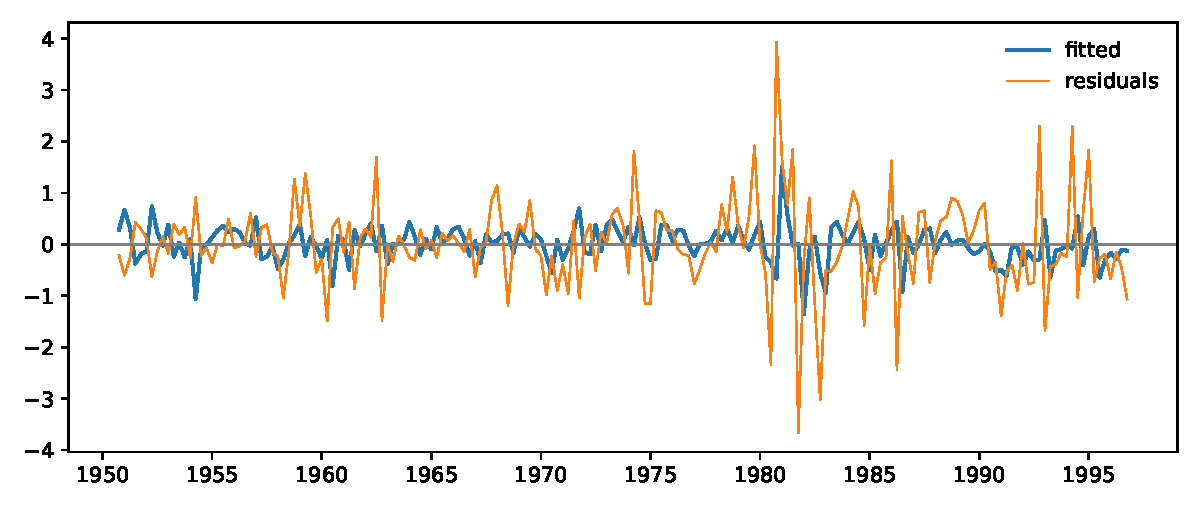
\includegraphics[width=0.9\textwidth]{../LaTeX/hw01_q2_plot.pdf}\\
  {\small Fitted values and residuals, 1950:4--1996:4.}
\end{center}

Residuals on a constant and $\hat y$: both coefficients are zero (up to $10^{-16}$ rounding) and $R^{2} = 0$.

Fitted values on a constant and $e$: the slope is zero and $R^{2} = 0$; the intercept is $0.0134$, the mean of $\Delta r_{t}$.

\question{(3)}
Let $X_{1} = [\iota,\ \Delta y_{t-1},\ \Delta r_{t-1},\ \Delta r_{t-2}]$ and $x_{2} = \pi_{t-1}$.
Then $e_{t} = M_{1}\Delta r$, $e^{\pi}_{t} = M_{1}x_{2}$, and regressing $e_{t}$ on $e^{\pi}_{t}$ gives
\[
  \hat\beta = (x_{2}\xT M_{1}x_{2})^{-1}x_{2}\xT M_{1}\Delta r = 0.0161,
\]
the same as the coefficient on $\pi_{t-1}$ in (1).
The residuals are identical to the residuals from (1) (largest difference $9\times10^{-15}$).

\question{(4)}
Sample 1953:1--1996:4, $n = 176$, with $c_{t} = \log CE_{t}$ and $y_{t} = \log YD_{t}$. OLS gives
\[
  \widehat{\Delta c}_{t} = \underset{(0.0012)}{0.0051}
  + \underset{(0.0545)}{0.3058}\,\Delta y_{t}
  + \underset{(0.0544)}{0.1242}\,\Delta y_{t-1}
  + \underset{(0.0551)}{0.0425}\,\Delta y_{t-2}
  + \underset{(0.0545)}{0.1239}\,\Delta y_{t-3}
  - \underset{(0.0539)}{0.1233}\,\Delta y_{t-4}.
\]

Method 1. Let $w = (0,1,1,1,1,1)\xT$. Then
\[
  \hat\gamma = w\xT\hat\beta = 0.4732, \qquad
  \operatorname{se}(\hat\gamma) = \sqrt{w\xT \widehat{\Var}(\hat\beta)\,w} = 0.1000.
\]

Method 2. Substitute $\beta_{2} = \gamma - \beta_{3} - \beta_{4} - \beta_{5} - \beta_{6}$ into (2):
\[
  \Delta c_{t} = \beta_{1} + \gamma\,\Delta y_{t}
  + \beta_{3}(\Delta y_{t-1} - \Delta y_{t})
  + \beta_{4}(\Delta y_{t-2} - \Delta y_{t})
  + \beta_{5}(\Delta y_{t-3} - \Delta y_{t})
  + \beta_{6}(\Delta y_{t-4} - \Delta y_{t}) + \text{errors}.
\]
The coefficient on $\Delta y_{t}$ is now $\gamma$. OLS gives $\hat\gamma = 0.4732$ with standard error $0.1000$.

\question{(5)}
Original regression: $\hat\beta_{2} = (X_{2}\xT M_{1}X_{2})^{-1}X_{2}\xT M_{1}y$, residuals $\hat u = M_{X}y$,
and $y = X_{1}\hat\beta_{1} + X_{2}\hat\beta_{2} + M_{X}y$.
Facts used: $P_{1}X_{1} = X_{1}$, $M_{1}X_{1} = 0$, $P_{X}X_{i} = X_{i}$, $M_{X}X_{i} = 0$, $M_{1}M_{X} = M_{X}$, $P_{1}P_{X} = P_{1}$;
all projections are symmetric and idempotent.

\medskip\noindent(a) $y = X_{2}\beta_{2} + u$.
\begin{align*}
  \tilde\beta_{2} &= (X_{2}\xT X_{2})^{-1}X_{2}\xT y \neq \hat\beta_{2},\\
  \tilde u &= y - X_{2}\tilde\beta_{2} = M_{2}y \neq M_{X}y.
\end{align*}
$\beta_{2}$: not the same. Residuals: not the same.

\medskip\noindent(b) $P_{1}y = X_{2}\beta_{2} + u$.
\begin{align*}
  \tilde\beta_{2} &= (X_{2}\xT X_{2})^{-1}X_{2}\xT P_{1}y \neq \hat\beta_{2},\\
  \tilde u &= P_{1}y - X_{2}\tilde\beta_{2} = M_{2}P_{1}y \neq M_{X}y.
\end{align*}
$\beta_{2}$: not the same. Residuals: not the same.

\medskip\noindent(c) $P_{1}y = P_{1}X_{2}\beta_{2} + u$.
\begin{align*}
  \tilde\beta_{2} &= (X_{2}\xT P_{1}P_{1}X_{2})^{-1}X_{2}\xT P_{1}P_{1}y = (X_{2}\xT P_{1}X_{2})^{-1}X_{2}\xT P_{1}y \neq \hat\beta_{2},\\
  \tilde u &= P_{1}y - P_{1}X_{2}\tilde\beta_{2} = P_{1}(y - X_{2}\tilde\beta_{2}) \neq M_{X}y.
\end{align*}
$\beta_{2}$: not the same. Residuals: not the same.

\medskip\noindent(d) $P_{X}y = X_{1}\beta_{1} + X_{2}\beta_{2} + u$.
\begin{align*}
  \tilde\beta &= (X\xT X)^{-1}X\xT P_{X}y = (X\xT X)^{-1}(P_{X}X)\xT y = (X\xT X)^{-1}X\xT y = \hat\beta
  \;\Rightarrow\; \tilde\beta_{2} = \hat\beta_{2},\\
  \tilde u &= P_{X}y - X\hat\beta = P_{X}y - P_{X}y = 0 \neq M_{X}y.
\end{align*}
$\beta_{2}$: the same. Residuals: not the same.

\medskip\noindent(e) $P_{X}y = X_{2}\beta_{2} + u$.
\begin{align*}
  \tilde\beta_{2} &= (X_{2}\xT X_{2})^{-1}X_{2}\xT P_{X}y = (X_{2}\xT X_{2})^{-1}(P_{X}X_{2})\xT y = (X_{2}\xT X_{2})^{-1}X_{2}\xT y \neq \hat\beta_{2},\\
  \tilde u &= P_{X}y - X_{2}\tilde\beta_{2} = M_{2}P_{X}y \neq M_{X}y.
\end{align*}
$\beta_{2}$: not the same (same as (a)). Residuals: not the same.

\medskip\noindent(f) $M_{1}y = X_{2}\beta_{2} + u$.
\begin{align*}
  \tilde\beta_{2} &= (X_{2}\xT X_{2})^{-1}X_{2}\xT M_{1}y \neq (X_{2}\xT M_{1}X_{2})^{-1}X_{2}\xT M_{1}y = \hat\beta_{2},\\
  \tilde u &= M_{1}y - X_{2}\tilde\beta_{2} = M_{2}M_{1}y \neq M_{X}y.
\end{align*}
$\beta_{2}$: not the same. Residuals: not the same.

\medskip\noindent(g) $M_{1}y = M_{1}X_{2}\beta_{2} + u$.
\begin{align*}
  \tilde\beta_{2} &= (X_{2}\xT M_{1}M_{1}X_{2})^{-1}X_{2}\xT M_{1}M_{1}y = (X_{2}\xT M_{1}X_{2})^{-1}X_{2}\xT M_{1}y = \hat\beta_{2},\\
  \tilde u &= M_{1}y - M_{1}X_{2}\hat\beta_{2}
  = M_{1}(X_{1}\hat\beta_{1} + X_{2}\hat\beta_{2} + M_{X}y) - M_{1}X_{2}\hat\beta_{2}
  = M_{1}M_{X}y = M_{X}y.
\end{align*}
$\beta_{2}$: the same. Residuals: the same.

\medskip\noindent(h) $M_{1}y = X_{1}\beta_{1} + M_{1}X_{2}\beta_{2} + u$.
Since $X_{1}\xT M_{1}X_{2} = (M_{1}X_{1})\xT X_{2} = 0$, the cross-product matrix is block diagonal, so
\begin{align*}
  \tilde\beta_{1} &= (X_{1}\xT X_{1})^{-1}X_{1}\xT M_{1}y = 0,\\
  \tilde\beta_{2} &= (X_{2}\xT M_{1}X_{2})^{-1}X_{2}\xT M_{1}y = \hat\beta_{2},\\
  \tilde u &= M_{1}y - X_{1}\cdot 0 - M_{1}X_{2}\hat\beta_{2} = M_{X}y \quad\text{(as in (g))}.
\end{align*}
$\beta_{2}$: the same. Residuals: the same.

\medskip\noindent(i) $M_{1}y = M_{1}X_{1}\beta_{1} + M_{1}X_{2}\beta_{2} + u$.
Since $M_{1}X_{1} = 0$, the $X_{1}$ block is all zeros and $\beta_{1}$ is not identified; the regression reduces to (g):
\begin{align*}
  \tilde\beta_{2} &= (X_{2}\xT M_{1}X_{2})^{-1}X_{2}\xT M_{1}y = \hat\beta_{2},\\
  \tilde u &= M_{1}y - M_{1}X_{2}\hat\beta_{2} = M_{X}y.
\end{align*}
$\beta_{2}$: the same. Residuals: the same.

\medskip\noindent(j) $P_{X}y = M_{1}X_{2}\beta_{2} + u$.
Here $M_{1}P_{X}y = M_{1}(X_{1}\hat\beta_{1} + X_{2}\hat\beta_{2}) = M_{1}X_{2}\hat\beta_{2}$, so
\begin{align*}
  \tilde\beta_{2} &= (X_{2}\xT M_{1}X_{2})^{-1}X_{2}\xT M_{1}P_{X}y = (X_{2}\xT M_{1}X_{2})^{-1}X_{2}\xT M_{1}X_{2}\hat\beta_{2} = \hat\beta_{2},\\
  \tilde u &= P_{X}y - M_{1}X_{2}\hat\beta_{2} = X_{1}\hat\beta_{1} + P_{1}X_{2}\hat\beta_{2} = P_{1}(X_{1}\hat\beta_{1} + X_{2}\hat\beta_{2}) = P_{1}P_{X}y = P_{1}y \neq M_{X}y.
\end{align*}
$\beta_{2}$: the same. Residuals: not the same.

\medskip\noindent
$\beta_{2}$ is the same in (d), (g), (h), (i), (j). The residuals are the same only in (g), (h), (i).

\end{document}
